\documentclass[10pt,twocolumn,twoside,letterpaper]{IEEEtran}

\usepackage[spanish]{babel}
\usepackage{amsmath}
\usepackage{graphics}
\usepackage{graphicx}
\usepackage{color}
\usepackage{anysize}

%\setlength{\oddsidemargin}{1cm}
%\setlength{\evensidemargin}{0.25mm}
%\setlength{\topmargin}{0.37cm}
\setlength{\textwidth}{15.6cm}
\setlength{\columnsep}{1.19cm}
\setlength{\textheight}{23cm}
%\pagestyle{headings} %%Encabezados

\marginsize {3.5cm}{2.5cm}{3.2cm}{-.05cm}
\bibliographystyle{/home/rsheissa/papers/inaoe_investigation_2005/ieeebib}

%opening
\title{Paradigma de Programaci\'on Orientada a Objetos Aplicada al Dise\~no Estructurado de Amplificadores}
\author{\begin{Large}{Roberto Casta\~neda Sheissa}\end{Large}\\ \begin{Large}Instituto Nacional de Astrof\'isica, \'Optica y Electr\'onica\end{Large}\\ \begin {Large} Departamento de Electr\'onica, Grupo de CAD\end{Large}\\ \begin{Large}P.O. Box 51, 72000, Puebla, Pue., M\'exico\end{Large}\\ \begin{Large}Email: {\tt rsheissa@inaoep.mx}\end{Large}}

\begin{document}

\pagestyle{empty}
\maketitle

\thispagestyle{empty}
\begin{abstract}
Este trabajo tiene como finalidad el mostrar que es posible aplicar el concepto de programaci\'on orientada a objetos ({\bf POO}) utilizada por los desarrolladores de software en el \'area de dise\~no electr\'onico. La t\'ecnica de dise\~no electr\'onico conocida como {\it dise\~no estructurado} posee caracter\'isticas que lo pueden definir como un proceso orientado a objetos. 
\end{abstract}

{\section{\bf {INTRODUCCI\'ON}}
La programaci\'on orientada a objetos (POO) puede definirse de la siguiente forma \cite{booch}:
\begin{description}
\item{\it ``Programaci\'on orientada a objetos es un m\'etodo de implementaci\'on en el cual los programas est\'an organizados en colecciones de objetos cooperativos, en el cual cada uno representa una instancia de alguna clase, y cuyas clases son todas miembros de una jeraqu\'ia de clases unidas v\'ia las relaciones de herencia.''}
 \end{description}

Hay tres partes importantes que hacer notar de la anterior definici\'on: la programaci\'on o\-rien\-ta\-da a objetos (1) utiliza {\it objetos}, no algoritmos, como los bloques b\'asicos fundamentales; (2) \mbox{cada} objeto es una {\it instancia} de alguna {\it clase}; y (3) las clases se relacionan cada una v\'ia las relaciones de {\it herencia}.

Por otro lado el dise\~no orientado a objetos (DOO) se define \cite{booch}:
\begin{description}
\item {\it ``El dise\~no orientado a objetos es un m\'etodo de dise\~no que abarca el proceso de descomposici\'on orientado a objetos y una anotaci\'on para describir modelos tanto l\'ogicos y f\'isicos, como tambi\'en modelos est\'aticos y din\'amicos del sistema a dise\~nar''}. (Ver Figura \ref{fig:sd}).
\end{description}

\begin{figure}[hbtp]
	\centering
	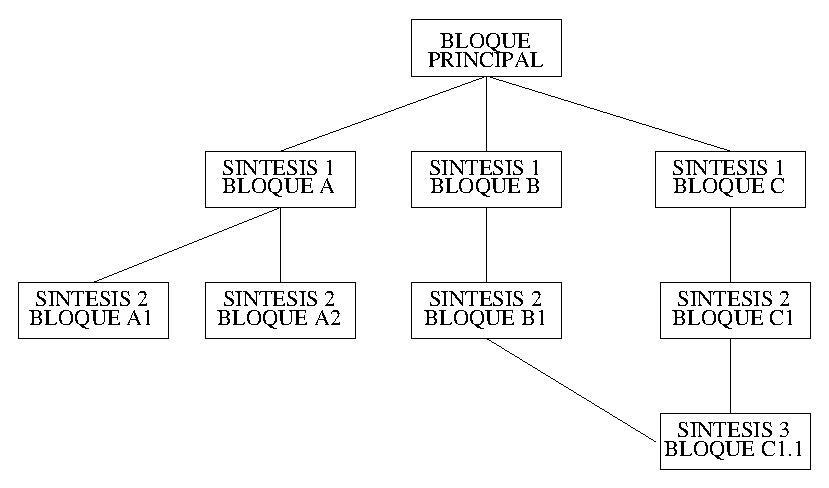
\includegraphics[height=2.25in,width=2.5in]{figures/ed.eps}
	\caption{Dise\~no Orientado a Objetos.}
	\label{fig:sd}
\end{figure}

Con respecto a la anterior definici\'on, es importante hacer notar lo siguiente: el dise\~no o\-rien\-ta\-do a objetos (1) gu\'ia a una descomposici\'on orientada a objetos y (2) utiliza di\-fe\-ren\-tes notaciones para expresar diferentes modelos del dise\~no l\'ogico (arquitectura de clases y objetos) y del dise\~no f\'isico (arquitectura de m\'odulo y procesos) de un sistema.

El dise\~no orientado a objetos hace uso de clases y abstracciones de objetos para sistemas de estructura l\'ogica; el dise\~no estructurado utiliza abstracciones algor\'itmicas. El {\it modelo de objetos} est\'a conformado por cuatro elementos b\'asicos que permiten definir las bases sobre las cuales descansan los fundamentos de la POO, estos son \cite{joyanes},\cite{booch}:

\begin{itemize}
\item Abstracci\'on - Es la capacidad para examinar ``{\it algo}'' sin preocuparse de sus detalles internos. En un programa estructurado, es suficiente conocer la tarea espec\'ifica que hace un pro\-ce\-di\-mien\-to dado, y no es tan importante {\it c\'omo} se realiza es tarea.
\item Encapsulado - Tambi\'en conocido como {\it ocultaci\'on de la informaci\'on}, previene a otros objetos ver su interior, donde el comportamiento de la abstracci\'on se ha realizado. Una definici\'on m\'as espec\'ifica es \cite{booch}: ``encapsulado es el proceso de esconder todos los detalles de un objeto que no contribuye a sus caracter\'isticas esenciales''.
\item Modularidad - Aunque particionar un programa para reducir su complejidad es \'util, una mejor justificaci\'on para particionar un programa es que permite crear un cierto n\'umero de l\'imites bien definidos y documentados dentro del programa. {\it Modularidad} se define como ``la propiedad de un sistema que ha sido dividido en un conjunto de m\'odulos cohesivos y libremente conectados''.
\item Jerarqu\'ia - La abstracci\'on es \'util pero es posible encontrar una gran cantidad de abs\-tra\-ccio\-nes distintas, tantas que no sea posible comprenderlas a la vez. Encapsulado tambi\'en ayuda proporcionando una forma de agrupar abstracciones l\'ogicamente relacionadas. Sin embargo todav\'ia no es suficiente. Un conjunto de abstracciones forman una jerarqu\'ia, la identificaci\'on de estas jerarqu\'ias en el dise\~no ayudan en gran manera para poder entender el pro\-ble\-ma. {\it Jerarqu\'ia} se define como ``un arreglo u ordenamiento de abstracciones''.
\end{itemize}

Para el caso del dise\~no estructurado de circuitos electr\'onicos el proceso consiste, so\-me\-ra\-men\-te, en dividir el problema en peque\~nos problemas que puedan ser atacados individualmente. Una vez que los problemas individuales se han resuelto, se vuelven a integrar dando \mbox{como} resultado al final una soluci\'on efectiva al problema en particular.

En las siguientes secciones se mostrar\'a que el dise\~no estructurado de circuitos electr\'onicos cumple con las bases de la POO. Esta forma de dise\~no permite reducir el tiempo para crear nuevas opciones de circuitos electr\'onicos.

\section{{\bf DISE\~NO ESTRUCTURADO}}
El dise\~no de circuitos elctr\'onicos consiste de una b\'usqueda a trav\'es de un gran cantidad de combinaciones de componentes con diferentes tipos de propiedades. Ser\'ia una gran inversi\'on de tiempo encontrar un circuito apto realizando b\'usquedas y pruebas extensivas con cada posible combinaci\'on de componentes disponibles. Es necesario establecer una estrategia a fin de encontrar una soluci\'on lo m\'as r\'apido posible. La estrategia utilizada ``normalmente'' es utilizar un circuito y por medio de cambios en los par\'ametros se encuentra una soluci\'on al pro\-ble\-ma que se plantea con nuevas especificaciones \cite{verhoeven}. La manera en que se comporte el circuito bajo ciertas circunstancias har\'an que el dise\~no encontrado sea implementado o desechado; en caso de que el dise\~no no sea \'util, el proceso vuelve a comenzar.

Aunque el utilizar la estrategia ``normal'' tarde o temprano generar\'a resultados \'utiles, e\-xis\-ten graves desventajas al utilizar esta estrategia:

\begin{itemize}
\item Esta estrategia nunca garantiza que se encuentra la soluci\'on {\it \'optima} al problema y no proporciona informaci\'on para saber que tan cerca se encuentra.
\item La relaci\'on entre par\'ametros de componentes y el desempe\~no del circuito nunca se hace completamente expl\'icito. De manera incidental el desempe\~no del circuito puede hacerse sensible a un par\'ametro irrelevante debido al hecho de que el circuito no es \'util para la aplicaci\'on.
\item Es muy complicado determinar lo que se de debe cambiar a un circuito cuando, por ejemplo, las especificaciones cambian.
\end{itemize}

Para crear el orden del caos que es el dise\~no de amplificadores, se separa el dise\~no en pro\-ble\-mas m\'as peque\~nos, ortogonales en la medida de lo posible, lo cual permite clarificar el problema y facilita la manera de atacarlo. El m\'etodo de {\it dise\~no electr\'onico estructurado} \cite{verhoeven,nordholt} permite encontrar {\bf UNA} soluci\'on al pro\-ble\-ma de dise\~no r\'apidamente (Figura \ref{fig:sd_1}). Sin embargo este es un m\'etodo que se basa en una cierta cantidad de suposiciones y en una cantidad limitada de reglas. Por lo tanto la aplicaci\'on pr\'actica del dise\~no electr\'onico estructurado nunca deber\'a dar pie a un rechazo dogm\'atico de los resultados obtenidos por los dise\~nos utilizados con la estrategia ``normal'' (o resultados obtenidos por medio de otra estrategia) ya que esto provocar\'ia un retraso en la evoluci\'on de la teor\'ia de dise\~no.

\begin{figure}[hbtp]
	\centering
	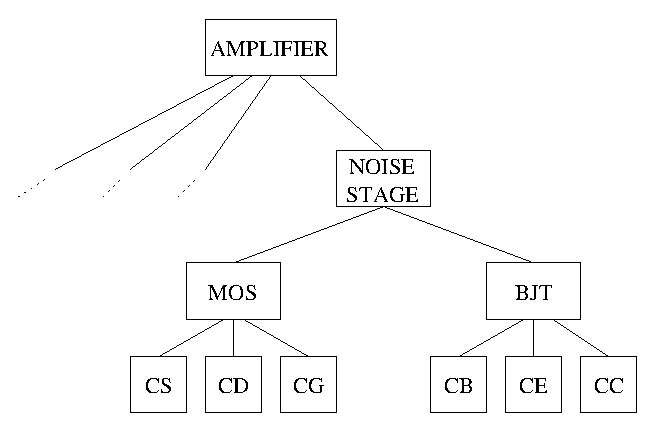
\includegraphics[scale=.65]{figures/bloque_ruido.eps}
	\caption{Ejemplo de Dise\~no Estructurado de Circuitos.}
	\label{fig:sd_1}
\end{figure}

El dise\~no estructurado de amplificadores se enfoca en tres aspectos fundamentales para realizar la descripci\'on del comportamiento del circuito:

\begin{itemize}
\item Ruido.
\item Distorsi\'on.
\item Ancho de Banda.
\end{itemize}

A fin de poder acelerar el proceso de dise\~no varias suposiciones deben de hacerse, como se dijo anteriormente. Estas se har\'an de acuerdo a las especificaciones b\'asicas que deben proporcionarse, en el comportamiento del circuito de acuerdo a los resultados obtenidos con modelos simples y a las decisiones que ata\~nen a cada etapa del dise\~no en particular. Este tipo de dise\~no se basa en tres elementos b\'asicos:

\begin{itemize}
\item Ortogonalidad - Los circuitos ser\'an ordenados de tal forma que el comportamiento de los tres aspectos fundamentales pueden ser dise\~nados ortogonalmente, es decir, el comportamiento de una etapa no tendr\'a influencia en las otras dos.
\item Simplicidad - Modelos simples se definen para obtener predicciones r\'apidas de la factibilidad del dise\~no. Soluciones no viables podr\'an ser detectadas en las primeras etapas del dise\~no. Una planificaci\'on especial se deber\'a hacer para permitir que los resultados ``estimados'' sean lo mas ``cercanos'' posibles a los valores reales.
\item Jerarqu\'ia - La jerarqu\'ia en el dise\~no permite reducir la complejidad del problema del dise\~no porque permite su divisi\'on eficiente en problemas de dise\~no m\'as peque\~nos e independientes. La planificaci\'on en este punto debe de ser a\-rre\-gla\-da de tal forma que las decisiones tomadas en un cierto nivel jer\'arquico se mantengan v\'alidas el resto del dise\~no.
\end{itemize}

\section{\bf RELACI\'ON CON POO}
Simplemente por el hecho de que la t\'ecnica de dise\~no electr\'onico contenga la frase ``estructurado'' no implica que cumpla con los principios b\'asicos del dise\~no orientado a objetos; en esta secci\'on se demuestra que no solo cumple la idea fundamental del DOO sino que tambi\'en se puede ampliar para poder trasladarse al POO y de esta manera poder crear una herramienta automatizada de dise\~no.

El dise\~no estructurado de circuitos electr\'onicos cumple con el principio de dise\~no o\-rien\-ta\-do a objetos ya que es un proceso que des\-com\-po\-ne un problema (bloque) en un cierto n\'umero de problemas m\'as peque\~nos (bloques), los cuales a su vez pueden ser subdivididos y as\'i sucesivamente hasta aislar un problema espec\'ifico. Con esto se demuestra que cumple con la definici\'on de DOO.

Una vez encontrada la relaci\'on con DOO, la atenci\'on se centrar\'a en llegar a demostrar que es posible llevar la idea del dise\~no estructurado hasta el concepto de POO. Un buen punto de partida es que ambas t\'ecnicas utilizan la idea de jerarqu\'ia en los dise\~nos, esto simplifica la factibilidad de proponer modelos jer\'arquicos que puedan ser convertidos en modelos \'utiles para POO. La complejidad de los modelos no deber\'a de cambiar, es decir, primero se utilizan modelos simples para pruebas preliminares y si estas pruebas resultan exitosas modelos complejos ser\'an sustituidos.

Para el concepto de abstracci\'on el dise\~no estructurado no tiene un concepto similar, sin embargo tiene un elemento que puede ser utilizado como un tipo de abstracci\'on. El nullor, elemento ideal sobre el cual parte la soluci\'on del pro\-ble\-ma de dise\~no puede ser considerado como el elemento de abstracci\'on. Este se tomar\'ia como {\bf abstracci\'on de entidad} \cite{booch}, se refiere a que un objeto representa un modelo \'util dentro del dominio del problema. En el caso de la POO su enfoque en este punto tambi\'en es utilizar la abstracci\'on de entidad.

La modularidad de la POO tiene su contrapartida en dise\~no estructurado en la or\-to\-go\-na\-li\-dad. El dise\~no se divide en tres partes para rea\-li\-zar la s\'intesis del nullor (ruido, ancho de banda y distorsi\'on). Una vez realizada la divisi\'on es posible subdividir cada una de las partes. Una vez que los peque\~nos problemas han \mbox{sido} resueltos se procede otra vez a ``aglutinar'' de nueva cuenta las partes hasta completar el bloque principal (el nullor sintetizado). Con \mbox{esto} se cumple la definici\'on de modularidad en POO. (Figura \ref{fig:nullor_1}). 

\begin{figure}[hbtp]
	\centering
	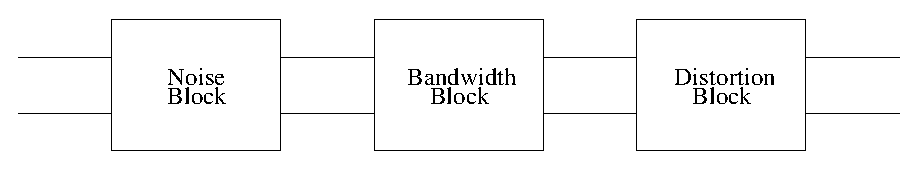
\includegraphics[height=.65in,width=2.8in]{figures/basic_blocks.eps}
	\caption{Divisi\'on en m\'odulos para sintetizar.}
	\label{fig:nullor_1}
\end{figure}

El encapsulado para el dise\~no estructurado es un concepto no muy aplicable en el sentido estricto del concepto. Una alternativa puede ser nuevamente el nullor y las diferentes etapas de su s\'intesis. El nullor es un elemento ideal que no existe  por lo que es necesario implementarlo utilizando dispositivos ``reales''. Al sintetizar la primera etapa (ruido) en la jerarqu\'ia m\'as alta se sigue viendo el nullor dentro del circuito de amplificaci\'on, al agregar el segundo bloque sintetizado (distorsi\'on) se sigue viendo como un solo bloque. Dentro de este nullor se encuentran los dispositivos activos (BJT's, MOSFET's) pero a una jerarqu\'ia m\'as baja. De esta manera es posible ``esconder'' todos los detalles de los objetos que forman parte de la implementaci\'on. (Figura \ref{fig:nullor}).

\begin{figure}[hbtp]
	\centering
	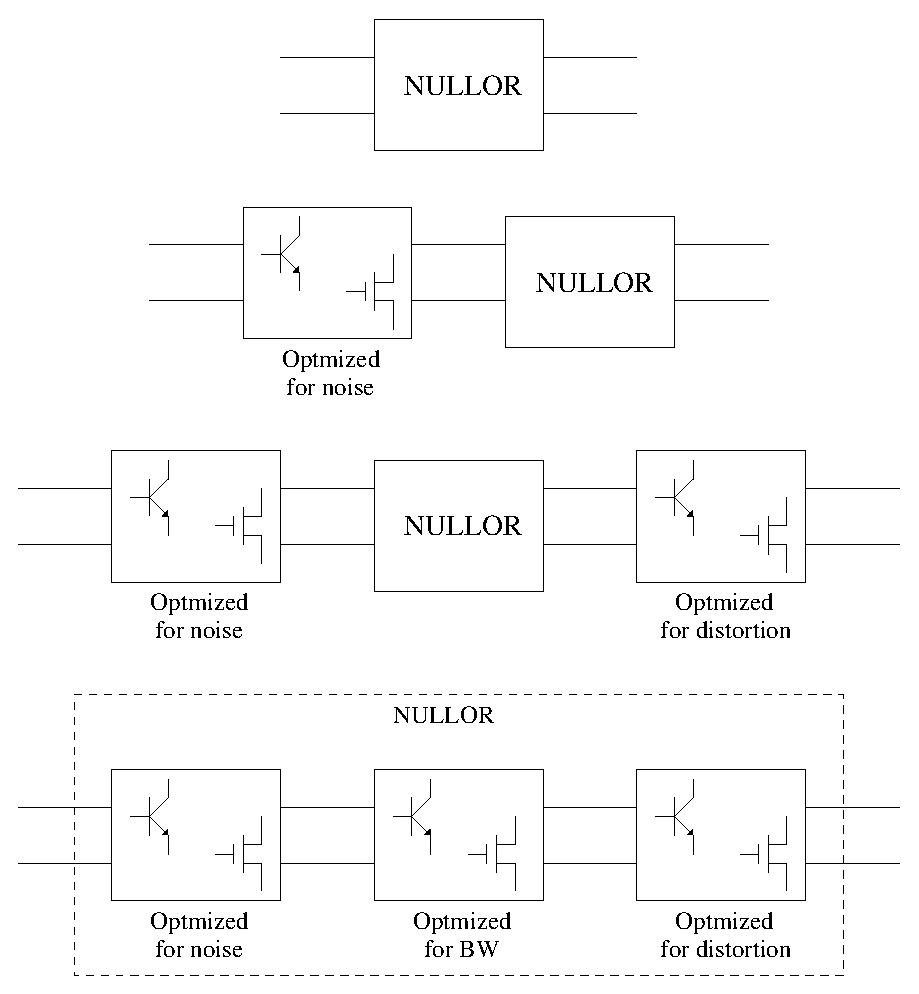
\includegraphics[scale=.5]{figures/synthesis_process.eps}
	\caption{Encapsulado aplicado a la s\'intesis del nullor.}
	\label{fig:nullor}
\end{figure}

\vspace*{-.37in}
\begin{center}
\begin{small}Fase a fase de dise\~no.\end{small}
\end{center}

\section{{\bf CONCLUSIONES}}
Es posible establecer una relaci\'on entre el dise\~no estructurado de circuitos electr\'onicos y la programaci\'on orientada a objetos. Los conceptos pueden ``adaptarse'' a fin de cumplir con los par\'ametros b\'asicos de la POO.

Una aplicaci\'on pr\'actica de los conceptos explicados en este trabajo ser\'ia el realizar el proceso de dise\~no aplicando la teor\'ia del dise\~no estructurado y documentando cada paso. Al encontrar la soluci\'on a un problema de forma sa\-tis\-fac\-to\-ria lo procedente es generalizar el proceso, es decir, a partir de varias condiciones iniciales encontrar en forma exitosa un dise\~no para cada una de ellas. Establecido el proceso y demostrado su factibilidad en la pr\'actica, este proceso puede ser convertido a un programa orientado a objetos.

Para poder convertir el proceso de dise\~no en un programa se realizan las analog\'ias mostradas en este documento y posteriormente se rea\-li\-za la codificaci\'on en alg\'un lenguaje de programaci\'on como Pascal, C++, Common Lisp Object System (CLOS), Ada, Ruby o JAVA. Lo m\'as dif\'icil del proceso es poder identificar donde aplicar los conceptos de encapsulado y mdoularidad sin romper con los conceptos b\'asicos tanto del dise\~no estructurado como el de la POO.

\section{{\bf AGRADECIMIENTOS}}
El autor agradece al CONACYT el apoyo otorgado atrav\'es de la beca de estudios de Doctorado n\'umero 118652/120341, la cual sin \mbox{ella} no hubiera sido posible rea\-li\-zar esta labor de investigaci\'on tan importante. Tambi\'en deseo agradecer el apoyo de los Doctores \mbox{Arturo} Sarmiento Reyes y Luis Hern\'andez Mart\'inez por la direcci\'on y atenci\'on prestada para la re\-a\-li\-za\-ci\'on del presente trabajo.


\bibliography{/home/rsheissa/papers/inaoe_investigation_2005/bib/descad}
\end{document}